% Panduan untuk penulis, bukan bagian naskah. Merangkum metode penelitian dalam satu halaman gambar dan satu tabel.
% Angka diambil dari paper/final (design.tex, results.tex). Bila naskah berubah, perbarui berkas ini.
\documentclass[10pt,a4paper]{article}
\usepackage[a4paper,margin=1.6cm]{geometry}
\usepackage[T1]{fontenc}
\usepackage{lmodern}
\usepackage{microtype}
\usepackage{tikz}
\usetikzlibrary{arrows.meta,positioning,calc,fit,backgrounds}
\usepackage{tabularx,booktabs,array,xcolor,enumitem}
\usepackage[hidelinks]{hyperref}
\definecolor{cai}{RGB}{226,135,30}
\definecolor{cdet}{RGB}{40,100,170}
\definecolor{chum}{RGB}{40,140,80}
\definecolor{cgr}{RGB}{110,110,110}
\definecolor{cred}{RGB}{200,50,50}
\newcolumntype{L}{>{\raggedright\arraybackslash}X}
\pagestyle{empty}
\setlength{\parindent}{0pt}
\setlength{\parskip}{0.45em}
\tikzset{
  st/.style={draw=#1, fill=#1!9, rounded corners=3pt, line width=0.7pt, align=left, font=\small,
    inner xsep=7pt, inner ysep=5pt, text width=11.2cm},
  tag/.style={circle, fill=#1, text=white, font=\bfseries\small, minimum size=0.62cm, inner sep=0pt},
  note/.style={font=\footnotesize, text=cgr, align=left, text width=4.6cm},
  ar/.style={-{Stealth[length=2mm]}, line width=0.9pt, draw=cgr}
}

\begin{document}
{\Large\bfseries Metode penelitian dalam satu gambar}\\[-0.2em]
{\small Panduan untuk penulis. Tidak masuk naskah.}

\vspace{0.4em}
\begin{center}
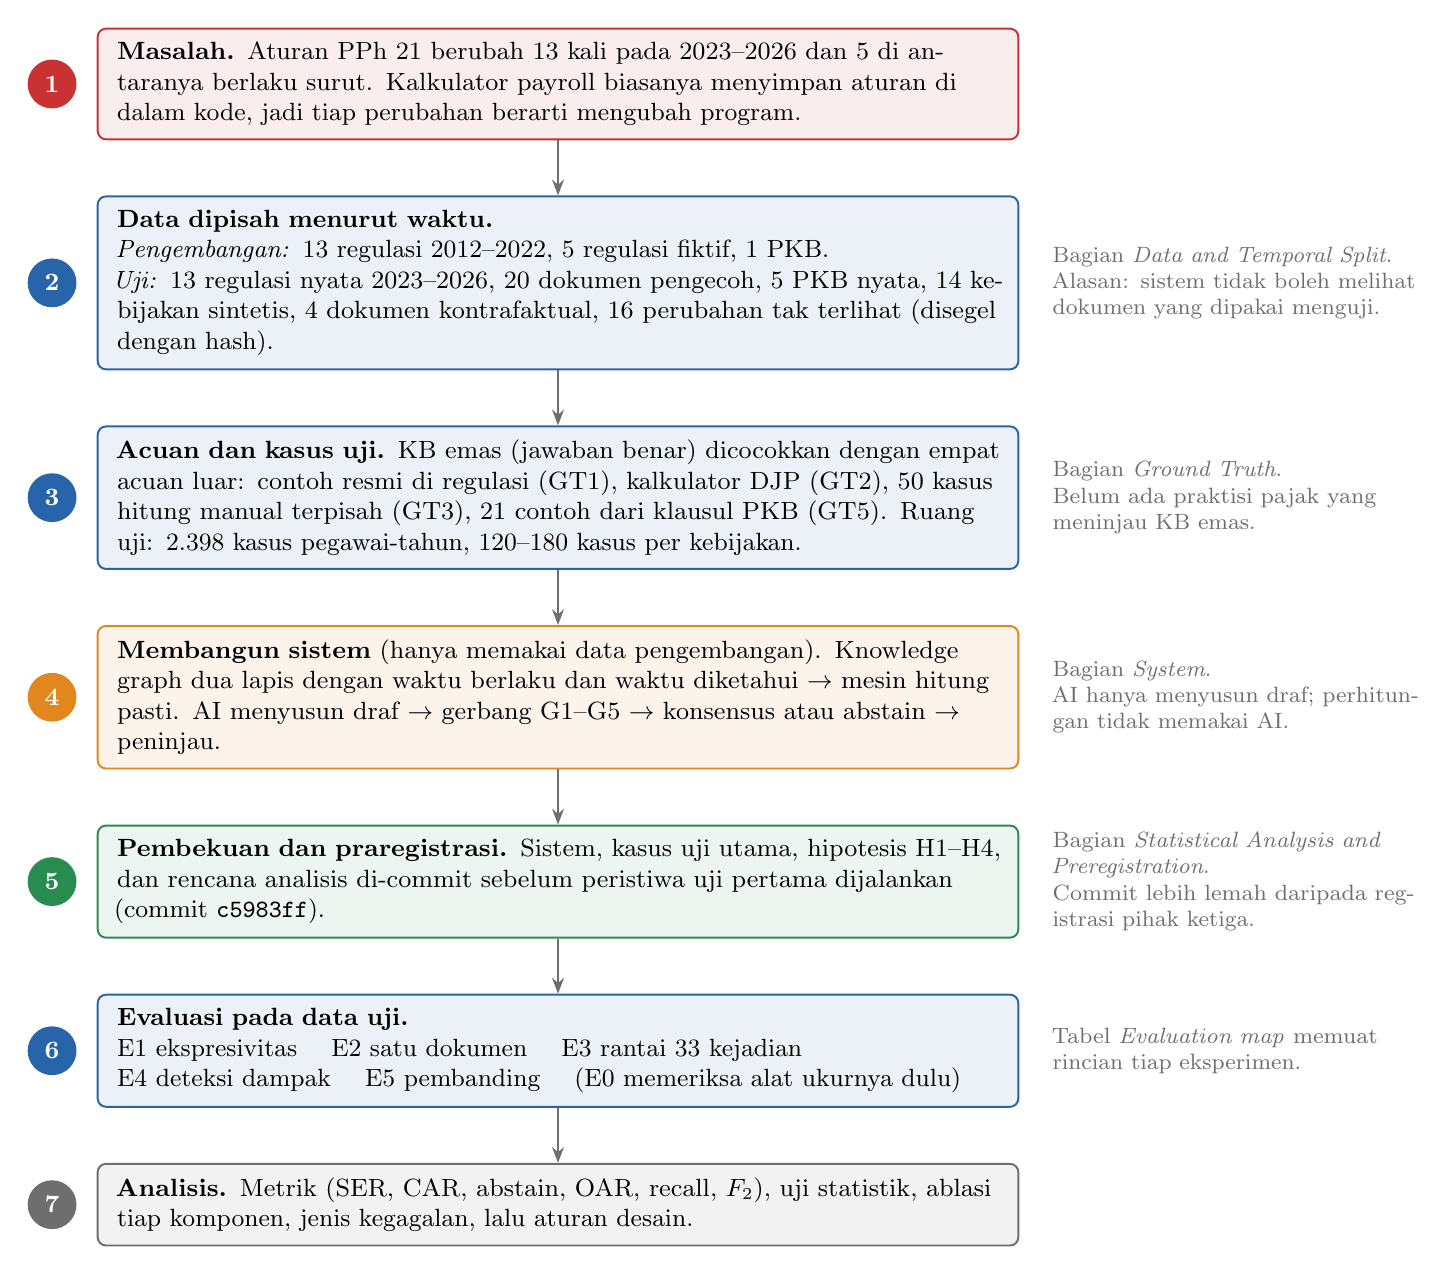
\begin{tikzpicture}[node distance=7mm]
\node[st=cred] (s1) {\textbf{Masalah.} Aturan PPh 21 berubah 13 kali pada 2023--2026 dan 5 di antaranya berlaku surut.
  Kalkulator payroll biasanya menyimpan aturan di dalam kode, jadi tiap perubahan berarti mengubah program.};
\node[st=cdet, below=of s1] (s2) {\textbf{Data dipisah menurut waktu.}\\
  \textit{Pengembangan:} 13 regulasi 2012--2022, 5 regulasi fiktif, 1 PKB.\\
  \textit{Uji:} 13 regulasi nyata 2023--2026, 20 dokumen pengecoh, 5 PKB nyata, 14 kebijakan sintetis,
  4 dokumen kontrafaktual, 16 perubahan tak terlihat (disegel dengan hash).};
\node[st=cdet, below=of s2] (s3) {\textbf{Acuan dan kasus uji.} KB emas (jawaban benar) dicocokkan dengan empat acuan luar:
  contoh resmi di regulasi (GT1), kalkulator DJP (GT2), 50 kasus hitung manual terpisah (GT3),
  21 contoh dari klausul PKB (GT5). Ruang uji: 2.398 kasus pegawai-tahun, 120--180 kasus per kebijakan.};
\node[st=cai, below=of s3] (s4) {\textbf{Membangun sistem} (hanya memakai data pengembangan).
  Knowledge graph dua lapis dengan waktu berlaku dan waktu diketahui $\rightarrow$ mesin hitung pasti.
  AI menyusun draf $\rightarrow$ gerbang G1--G5 $\rightarrow$ konsensus atau abstain $\rightarrow$ peninjau.};
\node[st=chum, below=of s4] (s5) {\textbf{Pembekuan dan praregistrasi.} Sistem, kasus uji utama, hipotesis H1--H4, dan rencana
  analisis di-commit sebelum peristiwa uji pertama dijalankan (commit \texttt{c5983ff}).};
\node[st=cdet, below=of s5] (s6) {\textbf{Evaluasi pada data uji.}\\
  E1 ekspresivitas \quad E2 satu dokumen \quad E3 rantai 33 kejadian\\
  E4 deteksi dampak \quad E5 pembanding \quad (E0 memeriksa alat ukurnya dulu)};
\node[st=cgr, below=of s6] (s7) {\textbf{Analisis.} Metrik (SER, CAR, abstain, OAR, recall, $F_2$), uji statistik, ablasi tiap
  komponen, jenis kegagalan, lalu aturan desain.};
\foreach \a/\b in {s1/s2,s2/s3,s3/s4,s4/s5,s5/s6,s6/s7}{\draw[ar] (\a.south)--(\b.north);}
\foreach \i/\c in {1/cred,2/cdet,3/cdet,4/cai,5/chum,6/cdet,7/cgr}{
  \node[tag=\c, anchor=east] at ($(s\i.west)+(-0.25,0)$) {\i};}
\node[note, anchor=west] at ($(s2.east)+(0.3,0)$) {Bagian \textit{Data and Temporal Split}.\\
  Alasan: sistem tidak boleh melihat dokumen yang dipakai menguji.};
\node[note, anchor=west] at ($(s3.east)+(0.3,0)$) {Bagian \textit{Ground Truth}.\\ Belum ada praktisi pajak yang meninjau KB emas.};
\node[note, anchor=west] at ($(s4.east)+(0.3,0)$) {Bagian \textit{System}.\\ AI hanya menyusun draf; perhitungan tidak memakai AI.};
\node[note, anchor=west] at ($(s5.east)+(0.3,0)$) {Bagian \textit{Statistical Analysis and Preregistration}.\\
  Commit lebih lemah daripada registrasi pihak ketiga.};
\node[note, anchor=west] at ($(s6.east)+(0.3,0)$) {Tabel \textit{Evaluation map} memuat rincian tiap eksperimen.};
\end{tikzpicture}
\end{center}

\newpage
{\Large\bfseries Lima eksperimen: yang ditanyakan dan hasilnya}

\vspace{0.3em}
\small
\begin{tabularx}{\textwidth}{@{}p{0.8cm} L p{3.3cm} L@{}}
\toprule
 & Pertanyaan sederhana & Data & Hasil (95\%, satu sisi bila disebut batas) \\
\midrule
E0 & Apakah alat ukur (KB emas dan kasus uji) bisa dipercaya? & 4 acuan luar, mutasi aturan & Tidak ada pelanggaran aturan dasar. Perbedaan dengan acuan dicatat satu per satu di lampiran. \\
E1 & Bisakah representasi memuat perubahan baru tanpa mengubah mesin? (H1, batas bawah $\geq 0{,}70$) & 16 perubahan tak terlihat & 16 dari 16 (batas bawah 0,829) setelah pembulatan contoh diseragamkan; tanpa itu hanya 8 dari 16. \textbf{Diterima dengan syarat.} \\
E2 & Seberapa aman satu usulan AI? (H2a, SER batas atas $\leq 0{,}25$; H2b, lebih baik dari B3 dan B4) & 13 regulasi + 5 PKB, 20 pengecoh & Benar 8, salah tanpa ketahuan 3, abstain 7 dari 18. SER batas atas 0,377. \textbf{Tidak diterima} (H2a dan H2b). \\
E3 & Apakah perubahan berurutan tetap stabil? (H3a, OAR $\geq 0{,}75$; H3b, galat terpicu dalam batas derau) & 33 kejadian berurutan & Rantai cangkok 31 dari 33, tetapi sebagian besar karena kasus sudah salah sejak awal. Rantai regenerasi 23 dari 33. H3a \textbf{diterima secara formal, rapuh}; H3b \textbf{tidak didukung}. \\
E4 & Bisakah sistem menemukan kebijakan perusahaan yang terdampak? (H4a, recall $\geq 0{,}70$; H4b, $F_2$ di atas dua pendeteksi sederhana) & 134 pasangan kebijakan--kejadian & Recall 0,91, presisi 0,71. H4a \textbf{diterima}; H4b \textbf{tidak diterima} (setara dengan menandai semua yang menyentuh fakta berubah). \\
E5 & Bagaimana dibanding cara lain? (deskriptif) & 2 kalkulator open-source, 100 kasus operasional & Kalkulator menambah TER 26 dan 915 hari setelah PP 58/2023; draf AI sekitar 12,5 menit (peninjauan tidak diukur). AI menghitung langsung tepat 76 dari 100 kasus, tanpa jejak. \\
\bottomrule
\end{tabularx}

\normalsize
\vspace{0.8em}
{\large\bfseries Yang perlu diingat saat menulis dan menjawab reviewer}
\begin{itemize}[leftmargin=1.2em, itemsep=0.2em]
\item \textbf{Kontribusi tidak bergantung pada hipotesis yang lolos.} Representasi, protokol replay, dan batas kemampuan AI
  (satu unsur selalu berhasil, 11 unsur ke atas tidak pernah) berdiri sendiri.
\item \textbf{Kelemahan terbesar:} KB emas dan 16 perubahan tak terlihat dibuat dan diperiksa agen AI dari keluarga model yang diuji,
  tanpa peninjau praktisi pajak. Naskah sudah menyebutnya sebagai keterbatasan.
\item \textbf{Praregistrasi memakai commit git} dan ada satu amandemen setelah hasil awal (commit \texttt{2df0727}).
  Hasil yang bergantung pada amandemen, selain pengecoh, putaran kedua, dan rantai regenerasi, ditandai eksploratori.
\item \textbf{Pengembangan v2 (8--9 November 2026)} memakai data pengembangan saja dan belum diuji dengan API.
  Hasilnya tidak masuk naskah sampai ada uji pada dokumen yang belum pernah dipakai.
\end{itemize}
\end{document}
